\beginsong{Die Mazurka}[
    wuw={Volkslied vom Balkan}, 
    txt={Marc-Andre Souchay}, 
    biest={531}, 
    bo={80}, 
    index={Mazurka},
]

\beginverse
\endverse
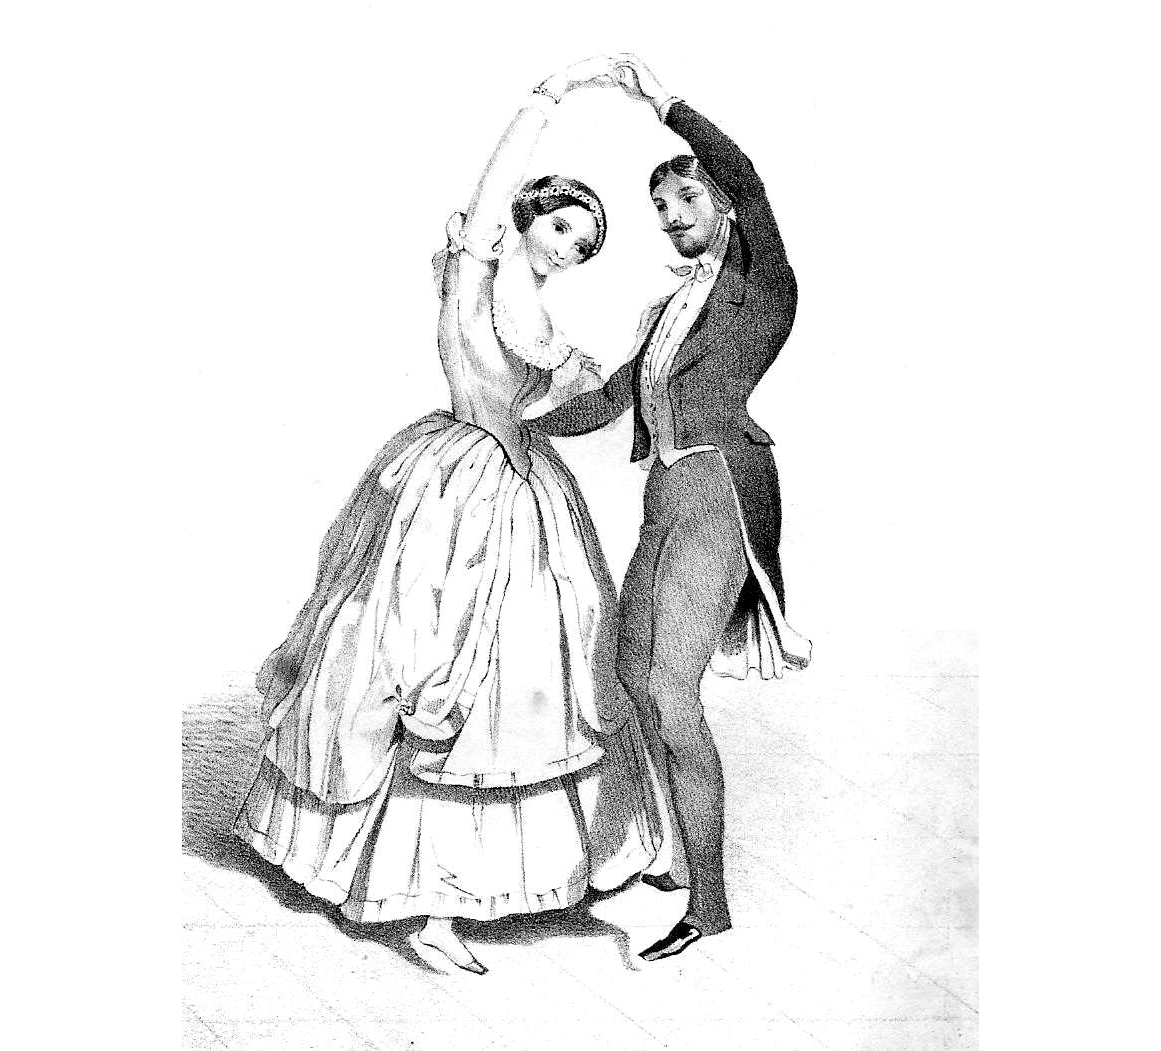
\includegraphics[page=1]{Noten/Mazurka.pdf}	

% \beginverse\memorize
% Die Maz\[Em]urk\[D]a \[G]lockt, \[D]Sie \[G]fährt uns in die \[H7]Glieder,
% jeder \[Em]Bursch \[D]springt \[G]auf \[D]und \[G]packt sein Lieb ums \[H7]Mieder.
% \lrep \[G]Tanzen wir, \[D]bis alleine \[Em]weiter wirbeln \[H7]Rock und Beine,
% falalala-\[Em]la la-\[H7]la la-\[Em]lalala, falalala-\[Em]la la-\[H7]la la-\[Em]la. \rrep
% \endverse

\beginverse\memorize
Unser \[Em]Vor\[D]bild \[G]ist \[D]der \[G]Borislav Schi\[H7]burka,
wie hat \[Em]er \[D]ge\[G]tanzt \[D]als \[G]König die Ma\[H7]zurka!
\[G]Borislav war \[D]schön wie keiner, \[Em]gut wie keiner, \[H7]kühn wie keiner,
falalala-\[Em]la la la-\[H7]la la-\[Em]lala, falalala-\[Em]la la-\[H7]la la-\[Em]la
\[G]Borislav war \[D]schön wie keiner, \[Em]gut wie keiner, \[H7]kühn wie keiner,
falalala-\[Em]la la la-\[H7]la la-\[Em]la.
\endverse

\beginverse
Boris^lav ^ist ^tot ^er ^ward ins Grab ge^legt schon,
die Ma^zur^ka ^weckt ^ihn ^auf, dass er sich ^regt schon.
^Streichen werden ^alle Geigen, ^er wird aus dem ^Grabe steigen,
falalala-^la la la-^la la-^lala, falalala-^la la-^la la-^la.
^Streichen werden ^alle Geigen, ^er wird aus dem ^Grabe steigen,
falalala-^la la la-^la la-^la.
\endverse

\endsong

\beginscripture{}
Bei der Mazurka handelt es sich um einen alten Polnischen Volkstanz. 
\endscripture
